% ----------------------------------- 
% TODO : modifié ce début de fichier 
% 
% Ce dossier de spécification est fortement inspiré du dossier de spécification réalisé par Milo KOSON de l'année dernière
%
% Document modifié et adapté par Théo BENARD
%-----------------------------------
\documentclass[a4paper,11pt,titlepage,french]{article}
% classe de document pour LaTeX qui définit les paramètres généraux du document : 
    % a4paper : définit le format de papier sur lequel le document doit être imprimé (a4paper format standard)
    % 11pt : définit la taille de police de base à 11 points
    % titlepage : demande à LaTeX d'insérer une page de titre dans le document
    % french : Cette option indique à LaTeX que le document est rédigé en français
% TODO : \input{chemin vers le fichier de setup} 
    % le fichier de setup devra contenir l'ensemble des usepackage suivants et les variables globales
% ----------------
% LIBRAIRIES LATEX
% ----------------
\usepackage[main=french]{babel}
\usepackage[T1]{fontenc}
\usepackage{fontspec}
\usepackage{fancyhdr}
\usepackage{xspace, graphicx}
\usepackage{longtable}
\usepackage[table]{xcolor}
\usepackage{hyperref}
\usepackage{enumitem}

% To use animUML example.tex file
\usepackage[T1]{fontenc}
\usepackage{graphicx}
\usepackage[export]{adjustbox}
\usepackage{float}

\usepackage{caption}
\usepackage{lastpage}

%\usepackage[outdir=build/epstopdf/, update]{epstopdf}
%\usepackage{array}
%\usepackage{multirow}
%\usepackage{changepage}
%\usepackage{hyperref}
%\usepackage{refcount}
% ------------------
% VARIABLES GLOBALES
% ------------------
\newcommand{\version}{2.0}
\newcommand{\revision}{0}
\newcommand{\documentName}{Dossier de Conception}
\newcommand{\documentNameAbrev}{CONC}
\newcommand{\prose}{ProSE}
\newcommand{\creator}{Elisa DECLERCK}
\newcommand{\projectName}{Passerelle Android-CAN vers banc CAN réel ou simulé} % TODO
\newcommand{\annee}{2024}
\newcommand{\teamName}{CANvengers} 
\newcommand{\teamNumber}{B1}
\newcommand{\client}{KEREVAL}
\newcommand{\nomLogiciel}{CANgateway} 
\newcommand{\nomApplication}{CANdroid} 

\setcounter{secnumdepth}{4} % Pour avoir une numérotation jusqu'au niveau 4
\renewcommand{\theparagraph}{\thesubsubsection.\arabic{paragraph}} % Pour numéroter les paragraphes à partir du niveau 3
\makeatletter % Redéfinit la commande \paragraph pour qu'elle utilise les paramètres de formatage de la commande \subsubsection.
\renewcommand\paragraph{\@startsection{paragraph}{4}{\z@}%
    {-3.25ex \@plus -1ex \@minus -.2ex}%
    {1.5ex \@plus .2ex}%
    {\normalfont\normalsize\bfseries}}
\makeatother
\setlength{\parindent}{0pt} % Supprime l'indentation par défaut

% -------------------------------------------------------
% --------------------------
% PARAMETRES HEADER / FOOTER 
% --------------------------
\pagestyle{fancy} % permet de personnaliser l'apparence de l'en-tête et du pied de page de chaque page du document
\setlength{\hoffset}{-40pt} % définis la marge horizontale gauche
\setlength{\topmargin}{-25pt} % définis la marge supérieure 
\setlength{\headsep}{10pt} % définis l'espace vertical entre l'en-tête et le corps de texte 
\renewcommand{\headheight}{60pt} % redéfinis la hauteur de l'en-tête
\renewcommand{\headwidth}{450pt} %  redéfinis la largeur de l'en-tête
\setlength{\textwidth}{450pt} % définis la largeur du corps de texte
\setlength{\textheight}{604pt} %  définis la hauteur du corps de texte
\renewcommand{\footrulewidth}{0.1mm} % redéfinis la largeur de la ligne de séparation de pied de page
\fancyhf{} % vide les entêtes et pieds de page précédemment définis
    % HEADER %
    \fancyhead[LO]{\bf \includegraphics[width=80pt]{../figures/eseo.png}\\ % fancyhead - personnaliser l'en-tête avec 2 arguments : orientation "LO" pour "Left Odd" / contenu "\bf" pour texte en gras + "\includegraphics" inclure le logo de l'ESEO
        \medskip % ajoute espace vertical moyen (≃ 6 points)
        {\prose} équipe {\teamNumber} {\annee}} % texte en dessous de l'image de la partie gauche du pdf
    \fancyhead[RO]{\bf 
\includegraphics[width=90pt]{../figures/logo_kereval.png}\\ % fancyhead - personnaliser l'en-tête avec 2 arguments : orientation "RO" pour "Right Odd" / contenu "\bf" pour texte en gras + "\includegraphics" inclure le logo de l'entreprise
        {\small{Ref. {\documentNameAbrev}\_{\teamNumber}}}} % texte en dessous de l'image de la partie droite du pdf
    % FOOTER %
    \fancyfoot[LO]{\sl {\it Version {\version} - Révision {\revision}}} % fancyfoot - personnaliser le pied de page avec 2 arguments : position "LO" pour "Left Odd" / contenu "\sl" + "\it" pour texte en italique de la version et la révision
    \cfoot{\copyright {\annee} Droits réservés {\teamName}} % insérer texte au centre du pied de page
    \fancyfoot[RO]{\thepage/\pageref{LastPage}} % pied de page partie droite : numéro de page
% ------------------------------
% FIN PARAMETRES HEADER / FOOTER 
% ------------------------------
% --------------
% DEBUT DOCUMENT 
% --------------
\begin{document}
\sloppy % relâche les règles de justification de texte pour éviter des espaces trop larges
\renewcommand{\arraystretch}{1.3} % augmente la hauteur des lignes d'un tableau

%-----------------------------------------------
%   The titles of the parts
%-----------------------------------------------
\makeatletter
% Adds a sub-subparagraph level
\newcounter{subsubparagraph}[subparagraph]
\renewcommand\thesubsubparagraph{%
    \thesubparagraph.\@arabic\c@subsubparagraph}
\newcommand\subsubparagraph{%
    \@startsection{subsubparagraph}               % counter
    {6}                                           % level
    {0em}                                         % indentation
    {1em}                                         % before the title
    {1em}                                         % after the title
    {\normalsize\hspace{6em}\color{colorTitle}} % style (overloaded by the title format)
}
\newcommand\l@subsubparagraph{\@dottedtocline{6}{13em}{6em}}
\newcommand{\subsubparagraphmark}[1]{}
\providecommand*{\toclevel@subsubparagraph}{6}

\setcounter{tocdepth}{6}    % Allows the paragraph in the table of contents
\setcounter{secnumdepth}{6} % Allows the numbering of the sub-paragraph

\makeatother
% -------------------
% PAGE DE GARDE {p.1}
% -------------------
\begin{center} % centre le contenu de la commande
    \vspace*{2cm} % ajout d'espace
    \rule[0.5ex]{0.7\textwidth}{0.1mm}\\ % ajout ligne horizontale : décalage verticale "ex" / largeur de page "%" / épaisseur "mm"
    \vspace*{2mm} % ajout d'espace
        {\Huge {\textsc{\bf {\documentName}}}} % crée un titre : police en gras "\bf" / petites capitales "\textsc" / grande taille polile "\Huge" 
    \vspace{0.4cm}\\ % ajout d'espace / "\\" : retour à la ligne 
        {\large\bf {\prose} {\teamNumber} {\annee} - {\teamName}}\\ % crée un titre : police en gras "\bf" / taille de police relativement grande "\large"
    \vspace*{1mm}
        {\large\bf {\projectName}}\\ % crée un titre 
    \rule[0.5ex]{0.75\textwidth}{0.1mm}\\ % ajout ligne horizontale
    \vspace{2cm} 
    \begin{tabular}{|c|c|} % crée un tableau avec 2 colonnes 
        \hline % crée une ligne dans le tableau // & : séparateur colonne
            Responsable du document & {\creator}                      \\
            État du document        & En réalisation                  \\
            Version                 & {\version}                      \\
            Révision                & {\revision}                     \\
        \hline
    \end{tabular}
\end{center}
\vspace{3cm} 
% -------------------
% AVERTISSEMENT {p.1}
% -------------------
\noindent % supprime l'indentation automatique au début d'un paragraphe
\textbf{AVERTISSEMENT :} % titre avertissement en gras
\vspace{3mm} \\
Le présent document est un document à but pédagogique.  
Le document de conception ci-joint est strictement confidentiel et réservé à un usage interne. 
Il a été réalisé sous la direction de Jérôme DELATOUR, en collaboration avec des enseignants 
et des étudiants de l'option SE du groupe ESEO. Ce document est la propriété de Jérôme DELATOUR, du groupe ESEO.
Toute utilisation, diffusion ou reproduction de ce document sans autorisation écrite préalable de Jérôme DELATOUR est interdite. 
Nous tenons à souligner que toute violation de cette politique pourrait engager la responsabilité civile et pénale de son auteur. 
Nous vous demandons de prendre toutes les précautions nécessaires pour assurer la sécurité et la confidentialité de ce document.
% -----------------------
% FIN PAGE DE GARDE {p.1}
% -----------------------
 
% ---------------------
% TABLEAU VERSION {p.2}
% ---------------------
% \noindent % Modifie l'espacement horizontal entre les colonnes
%
% Tableau des version à remplir à chaque fois que vous apportez une modification
%
\newpage % nouvelle page 
\begin{center}
\begin{longtable}[l]{|p{2cm}|p{5.8cm}|p{2.8cm}|p{1.4cm}|p{1.7cm}|}
    \hline
        \textbf{Date} & \textbf{Actions} & \textbf{Auteur} & \textbf{Version} & \textbf{Révision}\\
    \hline
        05/04/2023 & Création du document & Elisa\newline Declerck & 0.0 & 0\\
    \hline
        03/04/2023 & Réalisation du diagramme de séquence de "Démarrer le SàE" & Paul\newline  TRÉMOUREUX & 0.0 & 1 \\
    \hline
        07/04/2023 & Rédaction de Portée & Gabriel\newline MARQUETTE & 0.0 & 2\\
    \hline
        07/04/2023 & Rédaction de Objet & Gabriel\newline  MARQUETTE	& 0.0 & 3 \\
    \hline
        08/04/2023 & Réalisation de certains diagrammes de séquence & Théo\newline  BÉNARD & 0.0 & 4 \\	
    \hline
        10/04/2023 & Correction des diagrammes de séquence & Elisa\newline  DECLERCK & 0.0 & 5 \\	
    \hline
        12/04/2023 & Rédaction de la machine à états de Sender & Gabriel\newline  MARQUETTE & 0.0 & 6\\
    \hline
        12/04/2023 & Rédaction des descriptions des classes Sender, Basket et Network & Gabriel\newline  MARQUETTE & 0.0 & 7\\
    \hline
        12/04/2023 & Rédaction de la description générale des classes suivante : GUI, UI, Dealer, Logger, Object, Frame, Sniffer & Paul\newline  TRÉMOUREUX & 0.0 & 8\\
    \hline
        12/04/2023 & Rédaction de diagrammes de séquence & Thomas\newline  ROCHER & 0.0 & 9\\
    \hline
        12/04/2023 & Rédaction de diagrammes de séquence & Camille\newline  LENNE & 0.0 & 10\\
    \hline
        13/04/2023 & Correction du CU "Démarrer le SàE" & Paul\newline  TRÉMOUREUX & 0.0 & 11\\
    \hline
        13/04/2023 & Relecture et correction des doublons de descriptions générales de toutes les classes & Paul\newline  TRÉMOUREUX & 0.1 & 0\\
    \hline
        13/04/2023 & Rédaction de la description de l'architecture candidate & Elisa\newline  DECLERCK & 0.1 & 1\\
    \hline
	    13/04/2023 & Ajout des multiplicitées au diagramme de classe & Elisa\newline  DECLERCK & 0.1 & 2\\
    \hline
        15/04/2023 & Relecture des parties Références, Types de données et Services Offerts & Camille\newline LENNE & 0.1 & 3 \\
    \hline
        15/04/2023 & Relecture et correction de la description des diagrammes de séquence & Camille \newline LENNE & 0.1 & 4\\
    \hline
        16/04/2023 & Correction CU Reconnecter l'application {\nomApplication} & Thomas\newline  ROCHER & 0.1 & 5\\
    \hline
        16/04/2023 & Correction de la description de l'architecture candidate & Thomas\newline  ROCHER & 0.1 & 6\\
    \hline
        16/04/2023 & Inclusion de la MAE de GUI	& Elisa\newline  DECLERCK & 0.1 & 7 \\
    \hline
        17/04/2023 & Relecture section 2.2 + rédaction de note & Thomas\newline  ROCHER & 0.2 & 0\\		
    \hline
        17/04/2023 & Relecture partie + rédaction de note & Gabriel\newline  MARQUETTE & 0.2 & 1\\
    \hline
        17/04/2023 & Rédaction de la description de la MAE & Elisa\newline  DECLERCK & 0.2 & 2\\
    \hline
        18/04/2023 & Correction du schéma et de la description de la MAE de GUI & Elisa\newline  DECLERCK & 0.2 & 3\\
    \hline
        18/04/2023 & Correction de la section 2.2 & Thomas\newline  ROCHER & 0.2 & 4\\
    \hline
        19/04/2023 & Correction du dossier dans sa globalité & Théo\newline  BÉNARD & 1.0 & 0\\
    \hline
        26/04/2023 & Correction de certaines descriptions des diagrammes de séquence & Elisa\newline  DECLERCK & 1.0 & 1\\
    \hline
        27/04/2023 & Création de la MAE de UI et rédaction de sa description & Elisa\newline  DECLERCK & 1.0 & 2\\
    \hline
        27/04/2023 & Correction de la MAE de GUI & Gabriel\newline  MARQUETTE & 1.0 & 3\\
    \hline
        27/04/2023 & Correction de l'ensemble du dossier à la suite de l'audit consultatif & Elisa\newline  DECLERCK & 1.0 & 3\\
    \hline
        30/04/2023 & Relecture de la partie CANgateway de la conception détaillée & Thomas\newline  ROCHER & 1.1 & 0\\
    \hline
        24/05/2023 & Ajout de l'architecture du programme {\nomLogiciel} & Elisa\newline  DECLERCK & 1.1 & 1\\
    \hline
        26/05/2023 & Correction de la MAE de GUI & Elisa \newline DECLERCK & 1.1 & 2\\
    \hline
        26/05/2023 & Rédaction de la description des classes du programme {\nomLogiciel} & Elisa \newline DECLERCK & 1.1 & 3\\
    \hline
        28/05/2023 & Rédaction de la description des classes proxyGUI, proxyLogger, Dispatcher et Postman du programme {\nomLogiciel} & Thomas \newline ROCHER & 1.1 & 4\\
    \hline
        30/05/2023 & Rédaction des différents diagrammes de classes & Gabriel \newline MARQUETTE & 1.1 & 5 \\    
    \hline
        30/05/2023 & Rédaction du protocole de communication & Thomas \newline ROCHER & 1.1 & 6 \\    
    \hline
        31/05/2023 & Relecture de la conception détaillée & Thomas \newline ROCHER & 1.2 & 0 \\    
    \hline
        05/06/2023 & Correction dossier de conception & Elisa \newline DECLERCK & 1.2 & 1 \\
    \hline
        05/06/2023 & Correction et relecture de la conception détaillée coté Android & Camille \newline LENNE & 1.2 & 2 \\
    \hline
        09/06/2023 & Correction du dossier après audit normatif de code & Elisa \newline DECLERCK & 1.2 & 3 \\
    \hline
        13/06/2023 & Correction du dossier de conception dans sa globalité & Thomas \newline ROCHER & 2.0 & 0 \\
    \hline

\end{longtable}

\captionof{table}{Table des évolutions et validations internes du document}
\end{center}
\newpage % nouvelle page 
% -------------------------
% FIN TABLEAU VERSION {p.2}
% -------------------------

% --------------
% SOMMAIRE {p.3}
% --------------
\tableofcontents % génére table des matières en fonction des commandes "\section{}"
% ------------------
% FIN SOMMAIRE {p.3}
% ------------------

% ------------------
% INTRODUCTION {p.4}
% ------------------
% Auteurs : Camille Constant, Paul Trémoureux

\section{Introduction}
\label{sec:intro}

\subsection{Contexte}
\label{sec:intro:contexte}

\noindent\begin{tabularx}{\linewidth}{|p{3.5cm}|X|}
\hline
{\bf Produit à tester :} & {\projet} - version {\versionProjet}\\
\hline
{\bf Type de produit :} & {\produit}.\\
\hline
{\bf Commanditaire :} & {\client}\\
\hline
{\bf Développeur :} & {\equipe}\\
\hline
{\bf Testeur :} & {\equipe}\\
\hline
\end{tabularx}

\subsection{Objet}
\label{sec:intro:objet}

Ce document décrit l'activité de test système qui sera menée par {\equipe} durant le projet {\projet} dans le but de valider le produit suivant : {\produit}. Il est rédigé sous la responsabilité du Responsable Qualité-Test (RQT), sous la direction du Chef de Projet (CdP), conformément au Plan d'Assurance Qualité Logicielle (PAQL) élaboré sous la responsabilité du RQT (cf. section~\ref{sec:eqTest}, Équipe de test).

\subsection{Portée} 
\label{sec:intro:portee}

Sont concernés par ce document :
\begin{itemize}
    \item les testeurs : afin que ceux-ci connaissent le périmètre des tests (ce qu'ils vont tester), l'environnement de test (comment les tests seront mis en {\oe}uvre) et le processus de test (comment s'y prendre et rendre compte des résultats lors de l'exécution des tests) ;
    \item les développeurs : à titre informatif, afin que ceux-ci sachent comment va être validée leur production ; à titre indicatif afin qu'ils sachent, par la description de la gestion des anomalies, comment ils s'interfaceront avec l'équipe de test ;
    \item le client : ce plan de test fait l'objet d'une contractualisation avec le client pour déterminer le périmètre des tests menés pour valider le produit livré et les niveaux d'acceptation de cette validation ;
    \item les auditeurs : ce plan de test, ainsi que son implication, feront l'objet d'audits par la société Formato.
\end{itemize}

\subsection{Copyright}
\label{sec:intro:copyright}
Cf. {\refPAQL} (section 1.3. Copyright).

\subsection{Présentation du système} 
\label{sec:intro:scope}

Le système développé est un ensemble de 2 programmes : une application Android nommé {\appliA} déployé sur un smartphone Android et un programme C nommé {\appliC} déployé sur une Raspberry Pi.
L'application {\appliA} sera relié au programme {\appliC} par un réseau TCP/IP. La Raspberry Pi sera connectée à un réseau CAN pour dialoguer avec Tableau de Bord (soit banc de test physique soit simulateur sur un PC).
Ce projet permettra d'envoyer des trames depuis l'application {\appliA} vers Tableau de Bord afin de piloter ce dernier à distance.

\subsection{Références}
\label{sec:intro:ref}

\subsubsection{Documents de référence internes}
\noindent\begin{tabularx}{\linewidth}{|p{3cm}|X|p{1.4cm}|X|}
\hline
\textbf{Ref.} & \textbf{Nom et auteur} & \textbf{Version} & \textbf{Source}\\
\hline
{\refSpec} & Dossier de spécifications - \newline {\equipe} & 2.0.0 & se2024-b1.doc/specification/livrables\\
\hline
%Si client impliqué dans le PAQL
{\refPAQL} & Plan d'Assurance Qualité Logiciel - {\rqt} & 1.0.0 & pdf sur le dépôt\\
\hline
\end{tabularx}

\subsubsection{Documents de référence externes}
\noindent\begin{tabularx}{\linewidth}{|p{2.8cm}|X|}
\hline
\textbf{Ref.} & \textbf{Nom} \\
\hline
[ISO-829-2008] & Documentation de test logiciel\\
\hline
[ISO/IEC/IEEE 29119-1:2022] & Ingénierie du logiciel et des systèmes - Essais du logiciel - Partie 1: Concepts généraux\\
\hline
\end{tabularx}

\subsection{Glossaire et abréviations}
\label{sec:intro:termes}

Ce sont les termes et abréviations nécessaires à la compréhension de l'activité de test (les termes techniques propres au projet seront indiqués dans le dossier de spécification).

\subsubsection{Abréviations}

\noindent\begin{longtable}[c]{|p{.20\textwidth}|p{.80\textwidth}|}
\hline
CdP & Chef de Projet\\
\hline
IHM & Interface Homme-Machine\\
\hline
PAQL & Plan Assurance Qualité Logicielle\\
\hline
RQT & Responsable Qualité et Test\\
\hline
\end{longtable}

\subsubsection{Glossaire}

\noindent\begin{longtable}[c]{|p{.20\textwidth}|p{.80\textwidth}|}
\hline
{\bf Campagne de test} & Activité qui consiste à dérouler un ensemble de jeux de test. Un dossier de test est produit à l'issue d'une campagne.\\
\hline
{\bf Cas de test} & Déclinaison d'un test précisant les valeurs utilisées pour les variables du test ainsi que les résultats attendus.\\
\hline
{\bf Dossier de test} & Ensemble documentaire qui contient la description des scénarios et des cas de tests, ainsi que l'exécution des jeux de test. Le dossier de test est le reflet d'une campagne de test. \\
\hline
{\bf Jeux de test} & Ensemble des scénarios et cas de tests permettant de tester un produit logiciel. L'enchaînement des cas et scénarios de tests est relatif à une stratégie de test précisée dans le plan de test.\\
\hline
{\bf Plan de test} & Document décrivant le déroulement d'un jeu de test : stratégie de test, critères d'arrêt, planification.\\
\hline
{\bf Scénarios de test} & Ensemble de cas de tests cohérents permettant de traiter un objectif fonctionnel.\\
\hline
{\bf Test d'intégration} & Vérification effectuée pour montrer des défauts dans les interfaces et interactions de composants ou systèmes intégrés.\\
\hline
{\bf Test de non régression} & Vérification qu'une nouvelle version du produit fonctionne sans dégradation (technique, fonctionnelle, performance) par rapport à la version précédente.\\
\hline
{\bf Test de validation} & Vérification que le produit est cohérent et complet par rapport aux spécifications fonctionnelles.\\
\hline
{\bf Test fonctionnel} & Test (vu de l'utilisateur) du bon fonctionnement d'un produit logiciel, d'une fonctionnalité ou d'une fonction de base. Vérification par rapport aux spécifications.\\
\hline
{\bf Test système} & Vérification que le système dans son ensemble est cohérent et complet par rapport aux spécifications fonctionnelles et techniques.\\
\hline
{\bf Test unitaire} & Vérification que les composants logiciels individuels sont cohérents et complets par rapport aux spécifications.\\
\hline
\end{longtable}

Voir également le \href{https://www.cftl.fr/wp-content/uploads/2018/10/Glossaire-des-tests-logiciels-v3_2F-ISTQB-CFTL-1.pdf}{[Glossaire CFTL/ISTQB des termes utilisés en tests de logiciels]}.\\

\subsection{Conformité}
\label{sec:intro:conf}

Ce plan de test est conforme aux normes~:

\begin{itemize}
    \item IEEE Std. 1012-1986
    \item ISO Std. 829-2008
    \item IEEE Std. 1008-1987
    \item ISO/IEC/IEEE 29119-1:2022
\end{itemize}
% --------------------------
% CONCEPTION GENERALE {p.TODO}
% --------------------------
% WARNING: automatically generated file that may be overwritten or removed at any time

\section{Conception générale}

\newcommand\macroSuffix{}
\input{../animUML/Passerelle_CAN-macros}


\subsection{Architecture candidate}

\begin{figure}[H]
	\centering
	\includegraphics[max width=\textwidth,max height=.9\textheight]{../animUML/Passerelle_CAN-context}
	\caption{Architecture candidate}
	\label{fig:archiCand}
\end{figure}
Le diagramme de la \autoref{fig:archiCand} représente l'architecture candidate du système.
\\

Il s'agit de la conception générale ; l'hypothèse d'un système matériel à ressources infinies est pour l'instant posée. 

\begin{itemize}
    \item Dans ce diagramme, on retrouve deux objets représentant des interfaces homme-machine : 
    \begin{itemize}
        \item \textit{ui}, permettant de démarrer ou arrêter le programme {\nomLogiciel} et d'informer Utilisateur du bon fonctionnement du programme 
        \item \textit{gui}, permettant de démarrer et arrêter l'application {\nomApplication}. Il permet aussi à Utilisateur de réaliser divers actions et d'afficher les écrans (EcranPrincipal et Popup).
    \end{itemize}

    \item L'objet \textit{dealer} stocke et fournit à \textit{gui} les informations nécessaires à l'affichage des écrans. Il peut ajouter de nouveaux objets ou trames ou supprimer des éléments sélectionnés par Utilisateur et stockés dans \textit{basket}.

    \item L'objet \textit{object} permet de stocker et récupérer les informations d'une instance d'un objet, tout comme l'objet \textit{frame} permettant de stocker et récupérer les informations d'une instance d'une trame.

    \item L'objet \textit{basket} contient l'ensemble des objets et des trames sélectionnés par Utilisateur.

    \item L'objet \textit{sender} permet d'envoyer les trames sélectionnées par Utilisateur et stockées dans \textit{basket}.

    \item L'objet \textit{sniffer} permet de récupérer les trames reçues par le bus CAN et de les stocker dans l'objet \textit{logger}. 

    \item L'objet \textit{logger} permet de stocker les trames reçues par le bus CAN et de notifier \textit{gui} qu'une nouvelle trame doit être affichée.

    \item L'objet \textit{network} permet d'informer \textit{gui} de l'état de connexion entre l'application {\nomApplication} et le programme {\nomLogiciel}.
\end{itemize}

\subsection{Diagrammes de séquence}

\subsubsection{\emph{CU Échanger des trames CAN}}
\begin{figure}[H]
	\centering
	\includegraphics[max width=\textwidth,max height=.9\textheight]{../animUML/Passerelle_CAN-sequence-CU_Échanger_des_trames_CAN}
	\caption{Diagramme de séquence du \emph{CU Échanger des trames CAN}}
	\label{fig:inter-CU_Échanger_des_trames_CAN}
\end{figure}
Le diagramme de la \autoref{fig:inter-CU_Échanger_des_trames_CAN} représente le diagramme de séquence du \emph{CU Échanger des trames CAN}.
\input{sections/2_Conception_generale/Description_sequences/CU_Échanger_des_trames_CAN.tex}

\subsubsection{\emph{CU Démarrer le SàE - Scénario nominal}}
\begin{figure}[H]
	\centering
	\includegraphics[max width=\textwidth,max height=.9\textheight]{../animUML/Passerelle_CAN-sequence-CU_Démarrer_le_SàE_-_Scénario_nominal}
	\caption{Diagramme de séquence du \emph{CU Démarrer le SàE - Scénario nominal}}
	\label{fig:inter-CU_Démarrer_le_SàE_-_Scénario_nominal}
\end{figure}
Le diagramme de la \autoref{fig:inter-CU_Démarrer_le_SàE_-_Scénario_nominal} représente le diagramme de séquence du \emph{CU Démarrer le SàE - Scénario nominal}.
\\
Pour rappel, en dehors de la portée du système, Utilisateur met en fonctionnement Tableau de Bord, connecte la Raspberry PI au bus CAN et met la Raspberry PI sous tension.\\
Utilisateur doit ensuite démarrer manuellement le programme {\nomLogiciel} via une connexion SSH avec la Raspberry PI. Quand le programme {\nomLogiciel} est démarré, la LED de la Raspberry PI renvoie l'information à Utilisateur. Le programme {\nomLogiciel} commence alors à lire les trames du bus CAN.\\
Ensuite, Utilisateur démarre l'application {\nomApplication} et EcranPrincipal s'affiche. L'application {\nomApplication} charge l'ensemble des éléments créés lors des précédentes utilisations et les affiche sur EcranPrincipal.\\
Enfin, l'application {\nomApplication} se connecte au programme {\nomLogiciel} et EcranPrincipal se met à jour.\\
Il est possible que la connexion entre l'application {\nomApplication} et le programme {\nomLogiciel} échoue. Dans ce cas, PopupReconnexion s'affiche et demande à Utilisateur s'il souhaite réessayer. Ce scénario n'est pas représenter sur la \autoref{fig:inter-CU_Démarrer_le_SàE_-_Scénario_nominal}.\\

\subsubsection{\emph{CU Reconnecter application CANdroid - Scénario nominal}}
\begin{figure}[H]
	\centering
	\includegraphics[max width=\textwidth,max height=.9\textheight]{../animUML/Passerelle_CAN-sequence-CU_Reconnecter_application_CANdroid_-_Scénario_nominal}
	\caption{Diagramme de séquence du \emph{CU Reconnecter application CANdroid - Scénario nominal}}
	\label{fig:inter-CU_Reconnecter_application_CANdroid_-_Scénario_nominal}
\end{figure}
Le diagramme de la \autoref{fig:inter-CU_Reconnecter_application_CANdroid_-_Scénario_nominal} représente le diagramme de séquence du \emph{CU Reconnecter application CANdroid - Scénario nominal}.
\input{sections/2_Conception_generale/Description_sequences/CU_Reconnecter_application_CANdroid_-_Scénario_nominal.tex}

\subsubsection{\emph{CU Recevoir des trames - Scénario nominal}}
\begin{figure}[H]
	\centering
	\includegraphics[max width=\textwidth,max height=.9\textheight]{../animUML/Passerelle_CAN-sequence-CU_Recevoir_des_trames_-_Scénario_nominal}
	\caption{Diagramme de séquence du \emph{CU Recevoir des trames - Scénario nominal}}
	\label{fig:inter-CU_Recevoir_des_trames_-_Scénario_nominal}
\end{figure}
Le diagramme de la \autoref{fig:inter-CU_Recevoir_des_trames_-_Scénario_nominal} représente le diagramme de séquence du \emph{CU Recevoir des trames - Scénario nominal}.
\input{sections/2_Conception_generale/Description_sequences/CU_Recevoir_des_trames_-_Scénario_nominal.tex}

\subsubsection{\emph{CU Interagir avec le sniffer - Scénario nominal}}
\begin{figure}[H]
	\centering
	\includegraphics[max width=\textwidth,max height=.9\textheight]{../animUML/Passerelle_CAN-sequence-CU_Interagir_avec_le_sniffer_-_Scénario_nominal}
	\caption{Diagramme de séquence du \emph{CU Interagir avec le sniffer - Scénario nominal}}
	\label{fig:inter-CU_Interagir_avec_le_sniffer_-_Scénario_nominal}
\end{figure}
Le diagramme de la \autoref{fig:inter-CU_Interagir_avec_le_sniffer_-_Scénario_nominal} représente le diagramme de séquence du \emph{CU Interagir avec le sniffer - Scénario nominal}.
\input{sections/2_Conception_generale/Description_sequences/CU_Interagir_avec_le_sniffer_-_Scénario_nominal.tex}

\subsubsection{\emph{CU Ajouter un objet - Scénario nominal}}
\begin{figure}[H]
	\centering
	\includegraphics[max width=\textwidth,max height=.9\textheight]{../animUML/Passerelle_CAN-sequence-CU_Ajouter_un_objet_-_Scénario_nominal}
	\caption{Diagramme de séquence du \emph{CU Ajouter un objet - Scénario nominal}}
	\label{fig:inter-CU_Ajouter_un_objet_-_Scénario_nominal}
\end{figure}
Le diagramme de la \autoref{fig:inter-CU_Ajouter_un_objet_-_Scénario_nominal} représente le diagramme de séquence du \emph{CU Ajouter un objet - Scénario nominal}.
\input{sections/2_Conception_generale/Description_sequences/CU_Ajouter_un_objet_-_Scénario_nominal.tex}

\subsubsection{\emph{CU Ajouter une trame - Scénario nominal}}
\begin{figure}[H]
	\centering
	\includegraphics[max width=\textwidth,max height=.9\textheight]{../animUML/Passerelle_CAN-sequence-CU_Ajouter_une_trame_-_Scénario_nominal}
	\caption{Diagramme de séquence du \emph{CU Ajouter une trame - Scénario nominal}}
	\label{fig:inter-CU_Ajouter_une_trame_-_Scénario_nominal}
\end{figure}
Le diagramme de la \autoref{fig:inter-CU_Ajouter_une_trame_-_Scénario_nominal} représente le diagramme de séquence du \emph{CU Ajouter une trame - Scénario nominal}.
\input{sections/2_Conception_generale/Description_sequences/CU_Ajouter_une_trame_-_Scénario_nominal.tex}

\subsubsection{\emph{CU Envoyer des trames - Scénario nominal}}
\begin{figure}[H]
	\centering
	\includegraphics[max width=\textwidth,max height=.9\textheight]{../animUML/Passerelle_CAN-sequence-CU_Envoyer_des_trames_-_Scénario_nominal}
	\caption{Diagramme de séquence du \emph{CU Envoyer des trames - Scénario nominal}}
	\label{fig:inter-CU_Envoyer_des_trames_-_Scénario_nominal}
\end{figure}
Le diagramme de la \autoref{fig:inter-CU_Envoyer_des_trames_-_Scénario_nominal} représente le diagramme de séquence du \emph{CU Envoyer des trames - Scénario nominal}.
\input{sections/2_Conception_generale/Description_sequences/CU_Envoyer_des_trames_-_Scénario_nominal.tex}

\subsubsection{\emph{CU Arrêter envoi des trames - Scénario nominal}}
\begin{figure}[H]
	\centering
	\includegraphics[max width=\textwidth,max height=.9\textheight]{../animUML/Passerelle_CAN-sequence-CU_Arrêter_envoi_des_trames_-_Scénario_nominal}
	\caption{Diagramme de séquence du \emph{CU Arrêter envoi des trames - Scénario nominal}}
	\label{fig:inter-CU_Arrêter_envoi_des_trames_-_Scénario_nominal}
\end{figure}
Le diagramme de la \autoref{fig:inter-CU_Arrêter_envoi_des_trames_-_Scénario_nominal} représente le diagramme de séquence du \emph{CU Arrêter envoi des trames - Scénario nominal}.
\\
Lorsque Utilisateur demande l'arrêt d'envoi des trames, l'application {\nomApplication} affiche PopupArretEnvoi. Utilisateur valide la demande d'arrêt, l'application {\nomApplication} stoppe l'envoi de trames et met à jour EcranPrincipal en conséquence.\\
Dans le cas général, si Utilisateur refuse la demande d'arrêt d'envoi des trames, l'application {\nomApplication} ne s'arrête pas et continue à envoyer des trames. Ce cas de figure est explicitement décrit dans le CU "Arrêter l'envoi des trames" du dossier de spécification [\hyperref[SPEC]{dossier\_de\_specification\_SPEC\_B1\_2024}].

\subsubsection{\emph{CU Supprimer un élément - Scénario nominal}}
\begin{figure}[H]
	\centering
	\includegraphics[max width=\textwidth,max height=.9\textheight]{../animUML/Passerelle_CAN-sequence-CU_Supprimer_un_élément_-_Scénario_nominal}
	\caption{Diagramme de séquence du \emph{CU Supprimer un élément - Scénario nominal}}
	\label{fig:inter-CU_Supprimer_un_élément_-_Scénario_nominal}
\end{figure}
Le diagramme de la \autoref{fig:inter-CU_Supprimer_un_élément_-_Scénario_nominal} représente le diagramme de séquence du \emph{CU Supprimer un élément - Scénario nominal}.
\\
Utilisateur sélectionne un objet et toutes les trames qui lui sont associées sont automatiquement sélectionnées en conséquence. Par la suite, L'application {\nomApplication} se met à jour. Après avoir sélectionné les éléments à supprimer, l'application {\nomApplication} affiche PopupSuppressionElement et Utilisateur valide la suppression. Une fois la suppression confirmée, l'application {\nomApplication} met à jour EcranPrincipal pour refléter les changements.\\

Dans le cas général, Utilisateur a la possibilité de sélectionner une trame sans nécessairement sélectionner l'objet qui la contient, et de la supprimer. De plus, il est possible de sélectionner plusieurs éléments simultanément pour les supprimer, et l'application {\nomApplication} met à jour EcranPrincipal en conséquence. Ces cas de figure ne sont pas présentés sur ce scénario, mais sont explicitement décrits dans le CU "Supprimer un élément" du dossier de spécification [\hyperref[SPEC]{dossier\_de\_specification\_SPEC\_B1\_2024}]. 

\subsubsection{\emph{CU Stopper le SàE - Scénario nominal}}
\begin{figure}[H]
	\centering
	\includegraphics[max width=\textwidth,max height=.9\textheight]{../animUML/Passerelle_CAN-sequence-CU_Stopper_le_SàE_-_Scénario_nominal}
	\caption{Diagramme de séquence du \emph{CU Stopper le SàE - Scénario nominal}}
	\label{fig:inter-CU_Stopper_le_SàE_-_Scénario_nominal}
\end{figure}
Le diagramme de la \autoref{fig:inter-CU_Stopper_le_SàE_-_Scénario_nominal} représente le diagramme de séquence du \emph{CU Stopper le SàE - Scénario nominal}.
\\ 
Pour arrêter le SàE, Utilisateur commence par arrêter l'application {\nomApplication} grâce à l'opération "stopCANdroid()". Il arrête ensuite le programme {\nomLogiciel} avec l'opération "stopCANgateway()". Cette opération se charge d'appeler l'opération "stopReading()" qui arrête la lecture en continue des trames CAN. Pour finir, le programme {\nomLogiciel} informe Utilisateur que le SàE est arrêté grâce à l'opération "signalState(programmeState : ProgrammeState). \\

Dans le cas général, Utilisateur peut décider d'utiliser seulement le Smartphone avec l'application {\nomApplication}, il n'a donc pas besoin d'arrêter le programme {\nomLogiciel}. \\


\subsection{Types de données}

\begin{figure}[H]
	\centering
	\includegraphics[max width=\textwidth,max height=.9\textheight]{../animUML/Passerelle_CAN-datatypes}
	\caption{Diagramme des types de données}
	\label{fig:datatypes}
\end{figure}
Le diagramme de la \autoref{fig:datatypes} représente les types de données utilisés.
\newline
\subsubsection{Description de l'énumération  IdScreenPopUp}

Cette énumération représente les différents types de pop-ups utilisés dans le système. Chaque valeur de l'énumération correspond à un type de pop-up spécifique, tel que, par exemple, l'ajout d'objet, l'arrêt d'envoi ou la demande de reconnexion.
\newline

En voici le détail des énumérations:
\enumIdScreenPopUpLiteralDescriptions

\subsubsection{Description de l'énumération ProgramState}

Cette énumération représente l'état du programme, qui peut être soit "OFF" lorsque le programme est arrêté, soit "ON" lorsque le programme est en cours d'exécution.
\newline

En voici le détail des énumérations:
\enumProgramStateLiteralDescriptions

\subsubsection{Description de l'énumération NetworkState}

Cette énumération représente l'état de la connexion réseau, qui peut être soit "CONNECTED" lorsque la connexion est établie, soit "NOT\_CONNECTED" lorsque la connexion est perdue.
\newline

En voici le détail des énumérations:
\enumNetworkStateLiteralDescriptions

\subsubsection{Description de l'énumération SenderMode}

Cette énumération représente le Mode Envoi des données, qui peut être soit "PUNCTUAL" pour un envoi ponctuel, soit "CYCLIC" pour un envoi cyclique.
\newline

En voici le détail des énumérations:
\enumSenderModeLiteralDescriptions

\subsubsection{Description de l'énumération SendingState}

Cette énumération représente l'état d'envoi des données, qui peut être soit "ON" lorsque l'envoi est activé, soit "OFF" lorsque l'envoi est désactivé.
\newline

En voici le détail des énumérations:
\enumSendingStateLiteralDescriptions

\subsubsection{Descriptions des autres types de données}

Voici une liste des autres types de données utilisés dans le dossier ainsi que leur description :
\begin{itemize}
    \item \textbf{bool} : booléen, peut prendre la valeur true ou false.
    \item \textbf{CANFrame} : structure de données représentant un trame CAN. Elle contient les champs suivants :
    \begin{itemize}
        \item \textbf{id} : identifiant de la trame. C'est un entier non signé de 32 bits.
        \item \textbf{size} : taille de la trame. C'est un entier non signé de 8 bits.
        \item \textbf{data} : tableau de 8 octets non signés contenant les données de la trame.
    \end{itemize}
    \item \textbf{IdElement} : identifiant des objets et des trames. C'est un entier non signé de 16 bits. L'ID d'un objet est de la forme XX000 où XX représente l'ID de l'objet. L'ID d'une trame est de la forme XXYYY où XX représente l'ID de l'objet et YYY représente l'ID de la trame. Par exemple, si l'objet "Clignotant droit" a pour ID 06000, alors la première trame associée à cet objet aura pour ID 06001.
    \item \textbf{String} : chaîne de caractères.
    \item \textbf{StructSenderMode} : structure de données contenant le Mode Envoi (enumération SenderMode) et la périodicité si le Mode Envoi est cyclique.
\end{itemize}

\subsection{Classes}

\subsubsection{Vue générale}

\begin{figure}[H]
	\centering
	\includegraphics[max width=\textwidth,max height=.9\textheight]{../animUML/Passerelle_CAN-classes}
	\caption{Diagramme de classes}
	\label{fig:classes}
\end{figure}
Le diagramme de la \autoref{fig:classes} représente les classes du système.

\subsubsection{La classe Utilisateur}

Le diagramme de la \autoref{fig:class-Utilisateur} représente la classe Utilisateur.
\begin{figure}[H]
	\centering
	\includegraphics[max width=\textwidth,max height=.9\textheight]{../animUML/Passerelle_CAN-class-Utilisateur}
	\caption{Diagramme de la classe Utilisateur}
	\label{fig:class-Utilisateur}
\end{figure}
\input{sections/2_Conception_generale/Description_classes/Utilisateur.tex}

\paragraph{Attributs}
\classUtilisateurProperties
\paragraph{Services offerts}
\classUtilisateurOperations
\subsubsection{La classe GUI}

Le diagramme de la \autoref{fig:class-GUI} représente la classe GUI.
\begin{figure}[H]
	\centering
	\includegraphics[max width=\textwidth,max height=.9\textheight]{../animUML/Passerelle_CAN-class-GUI}
	\caption{Diagramme de la classe GUI}
	\label{fig:class-GUI}
\end{figure}
% ----------------------------
% Description de la classe GUI
% ----------------------------
% TODO :
\paragraph{Philosophie de conception}
La classe GUI permet de gérer les interfaces utilisateur de l'application {\nomApplication}.\\

\paragraph{Attributs}
\classGUIProperties
\paragraph{Services offerts}
\classGUIOperations
\paragraph{Description comportementale}
\begin{figure}[H]
	\centering
	\includegraphics[max width=\textwidth,max height=.9\textheight]{../animUML/Passerelle_CAN-gui-SM}
	\caption{Machine à états de \emph{GUI}}
	\label{fig:sm-gui}
\end{figure}
Le diagramme de la \autoref{fig:sm-gui} représente la machine à états de \emph{GUI}.
\newline
Lorsque l'application {\nomApplication} démarre, l'état par défaut de la MAE est l'état MainScreen. Entrer dans cet état appelle systématiquement l'opération pour afficher EcranPrincipal. Un certain nombre d'opérations peuvent être appelées dans cet état. Elles sont internes à l'état. \newline

L'application {\nomApplication} entre dans l'état Popup lorsque l'opération associée à l'apparition d'un pop-up est appelée. Entrer dans cet état appelle l'opération pour afficher le pop-up correspondant. L'appel de l'opération "rejectRequest()" permet de ramener l'application {\nomApplication} à l'état MainScreen. L'appel de l'opération "acceptRequest()" permet de ramener l'application {\nomApplication} à l'état MainScreen et de lancer l'opération correspondante à l'action de Utilisateur selon le pop-up qui était précédemment affiché sur Smartphone. 

\subsubsection{La classe UI}

Le diagramme de la \autoref{fig:class-UI} représente la classe UI.
\begin{figure}[H]
	\centering
	\includegraphics[max width=\textwidth,max height=.9\textheight]{../animUML/Passerelle_CAN-class-UI}
	\caption{Diagramme de la classe UI}
	\label{fig:class-UI}
\end{figure}
% ---------------------------
% Description de la classe UI
% ---------------------------
% TODO :
 \paragraph{Philosophie de conception}
La classe UI permet de gérer les interactions de Utilisateur avec le programme {\nomLogiciel}.\\

\paragraph{Attributs}
\classUIProperties
\paragraph{Services offerts}
\classUIOperations
\subsubsection{La classe Dealer}

Le diagramme de la \autoref{fig:class-Dealer} représente la classe Dealer.
\begin{figure}[H]
	\centering
	\includegraphics[max width=\textwidth,max height=.9\textheight]{../animUML/Passerelle_CAN-class-Dealer}
	\caption{Diagramme de la classe Dealer}
	\label{fig:class-Dealer}
\end{figure}
% -------------------------------
% Description de la classe Dealer
% -------------------------------
% TODO :
 \paragraph{Philosophie de conception}
La classe Dealer permet de gérer les objets et trames enregistrés sur l'application {\nomApplication}.\\

\paragraph{Attributs}
\classDealerProperties
\paragraph{Services offerts}
\classDealerOperations
\subsubsection{La classe Logger}

Le diagramme de la \autoref{fig:class-Logger} représente la classe Logger.
\begin{figure}[H]
	\centering
	\includegraphics[max width=\textwidth,max height=.9\textheight]{../animUML/Passerelle_CAN-class-Logger}
	\caption{Diagramme de la classe Logger}
	\label{fig:class-Logger}
\end{figure}
% -------------------------------
% Description de la classe Logger
% -------------------------------
% TODO :
 \paragraph{Philosophie de conception}
La classe Logger permet de mémoriser les trames reçues par Sniffer et de les enregistrer dans un fichier.\\

\paragraph{Attributs}
\classLoggerProperties
\paragraph{Services offerts}
\classLoggerOperations
\subsubsection{La classe Object}

Le diagramme de la \autoref{fig:class-Object} représente la classe Object.
\begin{figure}[H]
	\centering
	\includegraphics[max width=\textwidth,max height=.9\textheight]{../animUML/Passerelle_CAN-class-Object}
	\caption{Diagramme de la classe Object}
	\label{fig:class-Object}
\end{figure}
% -------------------------------
% Description de la classe Object
% -------------------------------
% TODO :
 \paragraph{Philosophie de conception}
La classe Object représente une instance d'un objet \textit{object}. Il est caractérisé par son nom, son ID et les trames qui lui sont associées. Par cette classe, on peut récupérer les trames qui lui sont associées, en ajouter de nouvelles ou en supprimer.\\

\paragraph{Attributs}
\classObjectProperties
\paragraph{Services offerts}
\classObjectOperations
\subsubsection{La classe Frame}

Le diagramme de la \autoref{fig:class-Frame} représente la classe Frame.
\begin{figure}[H]
	\centering
	\includegraphics[max width=\textwidth,max height=.9\textheight]{../animUML/Passerelle_CAN-class-Frame}
	\caption{Diagramme de la classe Frame}
	\label{fig:class-Frame}
\end{figure}
% ------------------------------
% Description de la classe Frame
% ------------------------------
% TODO :
 \paragraph{Philosophie de conception}
La classe Frame représente une instance de l'objet \textit{frame}. Elle est caractérisée par sa trame (de type CANFrame) et son Mode Envoi. Avec cette classe, on peut récupérer le Mode Envoi de la trame mais aussi le modifier.\\

\paragraph{Attributs}
\classFrameProperties
\paragraph{Services offerts}
\classFrameOperations
\subsubsection{La classe Sniffer}

Le diagramme de la \autoref{fig:class-Sniffer} représente la classe Sniffer.
\begin{figure}[H]
	\centering
	\includegraphics[max width=\textwidth,max height=.9\textheight]{../animUML/Passerelle_CAN-class-Sniffer}
	\caption{Diagramme de la classe Sniffer}
	\label{fig:class-Sniffer}
\end{figure}
% --------------------------------
% Description de la classe Sniffer
% --------------------------------
% TODO :
 \paragraph{Philosophie de conception}
La classe Sniffer gère la lecture des trames sur le bus CAN et l'envoi des trames lues vers l'application {\nomApplication}.\\

\paragraph{Attributs}
\classSnifferProperties
\paragraph{Services offerts}
\classSnifferOperations
\paragraph{Description comportementale}
\begin{figure}[H]
	\centering
	\includegraphics[max width=\textwidth,max height=.9\textheight]{../animUML/Passerelle_CAN-sniffer-SM}
	\caption{Machine à états de \emph{Sniffer}}
	\label{fig:sm-sniffer}
\end{figure}
Le diagramme de la \autoref{fig:sm-sniffer} représente la machine à états de \emph{Sniffer}.
\newline
Lors du lancement de l'application {\nomApplication}, la machine à états est dans l'état IDLE. Dès que l'ensemble des connexions entre le Smartphone, la Raspberry PI et Tableau de Bord sont faites, la machine à états passe à l'état Listening. Dans cet état, Sniffer reçoit les trames en continu, comme le montre la fonction "receiveFrame()". \newline
Lorsque Utilisateur souhaite mettre en pause l'arrivée des trames, la machine repasse dans l'état IDLE via l'opération "stopListening()". Il peut ainsi retourner en écoute lors de la reprise du sniffer via l'opération "startListening()". \newline 
\subsubsection{La classe Network}

Le diagramme de la \autoref{fig:class-Network} représente la classe Network.
\begin{figure}[H]
	\centering
	\includegraphics[max width=\textwidth,max height=.9\textheight]{../animUML/Passerelle_CAN-class-Network}
	\caption{Diagramme de la classe Network}
	\label{fig:class-Network}
\end{figure}
% --------------------------------
% Description de la classe Network
% --------------------------------
% TODO :
 \paragraph{Philosophie de conception}
La classe Network permet d'interagir avec GUI et de déterminer si la connexion entre le smartphone et la Rapsberry Pi est établie. \\

\paragraph{Attributs}
\classNetworkProperties
\paragraph{Services offerts}
\classNetworkOperations
\subsubsection{La classe Basket}

Le diagramme de la \autoref{fig:class-Basket} représente la classe Basket.
\begin{figure}[H]
	\centering
	\includegraphics[max width=\textwidth,max height=.9\textheight]{../animUML/Passerelle_CAN-class-Basket}
	\caption{Diagramme de la classe Basket}
	\label{fig:class-Basket}
\end{figure}
% -------------------------------
% Description de la classe Basket
% -------------------------------
% TODO :
\paragraph{Philosophie de conception}
La classe Basket permet d'enregistrer les éléments sélectionnés par Utilisateur.\\

\paragraph{Attributs}
\classBasketProperties
\paragraph{Services offerts}
\classBasketOperations
\subsubsection{La classe Sender}

Le diagramme de la \autoref{fig:class-Sender} représente la classe Sender.
\begin{figure}[H]
	\centering
	\includegraphics[max width=\textwidth,max height=.9\textheight]{../animUML/Passerelle_CAN-class-Sender}
	\caption{Diagramme de la classe Sender}
	\label{fig:class-Sender}
\end{figure}
% -------------------------------
% Description de la classe Sender
% -------------------------------
% TODO :
 \paragraph{Philosophie de conception}
La classe Sender permet d'envoyer les trames sur le bus CAN.\\

\paragraph{Attributs}
\classSenderProperties
\paragraph{Services offerts}
\classSenderOperations
\paragraph{Description comportementale}
\begin{figure}[H]
	\centering
	\includegraphics[max width=\textwidth,max height=.9\textheight]{../animUML/Passerelle_CAN-sender-SM}
	\caption{Machine à états de \emph{Sender}}
	\label{fig:sm-sender}
\end{figure}
Le diagramme de la \autoref{fig:sm-sender} représente la machine à états de \emph{Sender}.
\newline
Lorsque l'application {\nomApplication} est en fonctionnement, la machine à états est dans l'état IDLE. L'opération "setSendingState()" renvoi la valeur de l'énumération correspondant à l'état d'envoi en cours. Ici, les trames ne sont pas envoyées sur Tableau de Bord, donc le retour est SENDING\_STATE\_OFF. \newline
Dès lors que Utilisateur souhaite envoyer des trames via l'opération "startSending()", la machine à états passe dans l'état Sending. État durant lequel, l'opération "setSendingState()" va retourner SENDING\_STATE\_ON afin d'informer que les trames sont en cours d'envoi, comme il est possible de le voir avec "do/send()" qui agit constamment. L'état est quitté lorsque l'opération "stopSending()" est appelée, cela arrête l'envoi des trames et remet l'état de la machine à états sur IDLE.\newline 

% --------------------------
% CONCEPTION DETAILLEE {p.TODO}
% --------------------------
\newpage
\section{Conception détaillée}

La conception détaillée définit l'architecture logique du système, c'est-à-dire :

\begin{itemize}
    \item répartir le système sur l'architecture matérielle.
    \item gérer les entrées/sorties et les IHM.
    \item élaborer les protocoles de communication.
    \item définir les parallélismes et l'initialisation.
    \item définir le démarrage, l'arrêt, et la destruction du SàE.
\end{itemize}

% Architecture physique
\subsection{Architecture physique}

Le diagramme ci-dessous représente l'architecture physique du programme {\nomLogiciel} et de l'application {\nomApplication} dans leur intégralité. En plus des
classes vues précédemment, ce diagramme présente la gestion de la communication ainsi que les objets frontières nécessaires au bon fonctionnement du système.
Dans ce diagramme, dans un souci de visibilité, nous avons décidé de ne pas détailler les opérations ainsi que les attributs des classes.

\begin{minipage}
    {\linewidth}
    \centering
    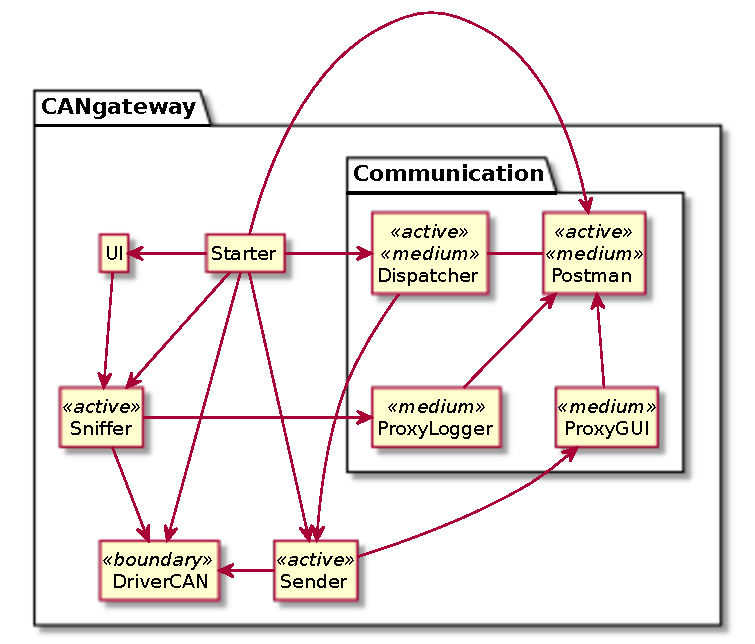
\includegraphics[width=0.8\textwidth]{../schemas/Conception_detaillee/architecture_CANgateway.pdf}
    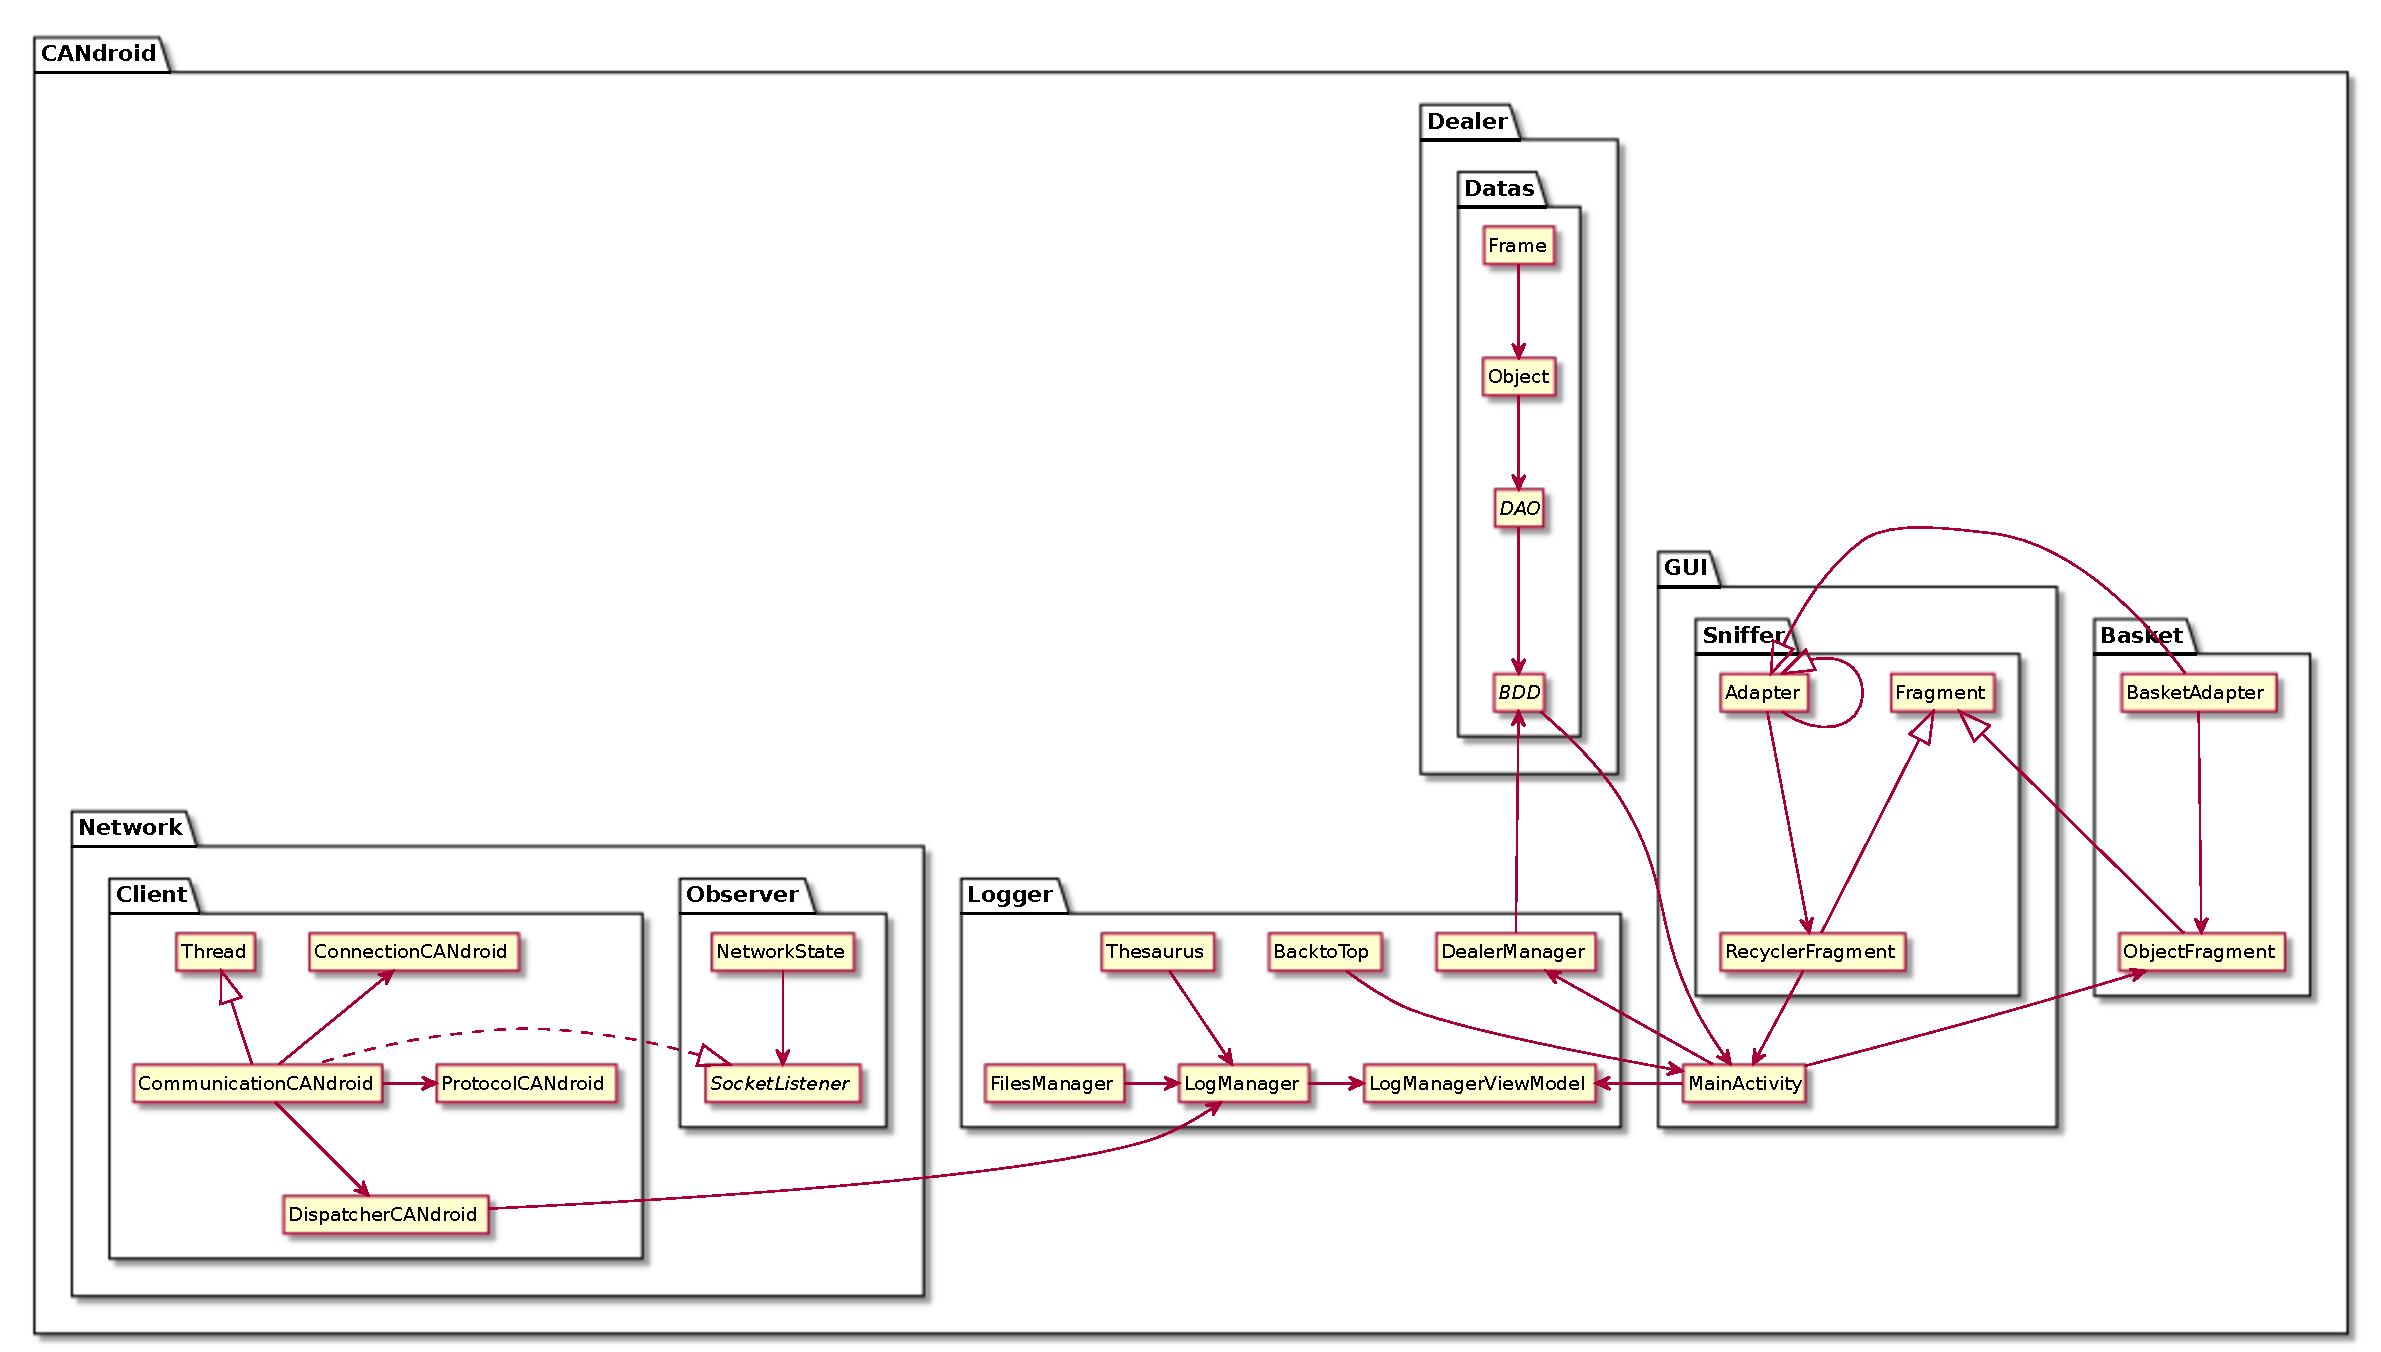
\includegraphics[width=\textwidth]{../schemas/Conception_detaillee/architecture_CANdroid.pdf}
    \captionof{figure}{Architecture physique}
\end{minipage}
\newpage 

% Description des classes
\subsection{Description des classes}

\subsubsection{Description des classes de CANdroid}

Suite à la conception générale, nous avons décidé de diviser certaines classes afin d'améliorer la lisibilité du programme de l'application {\nomApplication}, de faciliter sa réutilisation et son amélioration ultérieure. En effet, certaines classes de la conception générale, telles que Gui, Logger ou encore Basket, sont devenues des packages dans la conception détaillée. Le rôle du package dans la conception détaillée reste identique à celui des classes dans la conception générale. Bien qu'elles aient été divisées, nous fournirons néanmoins une description de chaque classe.

% Diagramme de classe de CANdroid
\input{sections/3_Conception_detaillee/2_Description_classes/1_Description_classes_CANdroid/description_diagramme_classe.tex}


%% Package Logger %%

% Diagramme de classe de Thesaurus
\input{sections/3_Conception_detaillee/2_Description_classes/1_Description_classes_CANdroid/description_classes_package_Logger/description_classe_thesaurus.tex}

% Diagramme de classe de FilesManager
\input{sections/3_Conception_detaillee/2_Description_classes/1_Description_classes_CANdroid/description_classes_package_Logger/description_classe_filesManager.tex}

% Diagramme de classe de LogManager
\input{sections/3_Conception_detaillee/2_Description_classes/1_Description_classes_CANdroid/description_classes_package_Logger/description_classe_LogManager.tex}

% Diagramme de classe de logMangerViewModel
\input{sections/3_Conception_detaillee/2_Description_classes/1_Description_classes_CANdroid/description_classes_package_Logger/description_classe_logManagerViewModel.tex}


%% Package Dealer

% Diagramme de classe de l'interface DAO
\input{sections/3_Conception_detaillee/2_Description_classes/1_Description_classes_CANdroid/description_classes_package_Dealer/description_interface_dao.tex}

% Diagramme de classe de BDD
\input{sections/3_Conception_detaillee/2_Description_classes/1_Description_classes_CANdroid/description_classes_package_Dealer/description_classe_bdd.tex}

% Diagramme de classe de Object
\input{sections/3_Conception_detaillee/2_Description_classes/1_Description_classes_CANdroid/description_classes_package_Dealer/description_classe_object.tex}

% Diagramme de classe de Frame
\input{sections/3_Conception_detaillee/2_Description_classes/1_Description_classes_CANdroid/description_classes_package_Dealer/description_classe_frame.tex}

% Diagramme de classe de Dealer
%\input{sections/3_Conception_detaillee/2_Description_classes/1_Description_classes_CANdroid/description_classes_package_Dealer/description_classe_dealer.tex}


%% Package Network

% Diagramme de classe de ProtocolCANdroid
\input{sections/3_Conception_detaillee/2_Description_classes/1_Description_classes_CANdroid/description_classes_package_Network/description_classes_protocolCANdroid.tex}

% Diagramme de classe de CommunicationCANdroid
\input{sections/3_Conception_detaillee/2_Description_classes/1_Description_classes_CANdroid/description_classes_package_Network/description_classe_communicationCANdroid.tex}

% Diagramme de classe de ConnectionCANdroid
\input{sections/3_Conception_detaillee/2_Description_classes/1_Description_classes_CANdroid/description_classes_package_Network/description_classe_connectionCANdroid.tex}

% Diagramme d'interface de SocketListener
\input{sections/3_Conception_detaillee/2_Description_classes/1_Description_classes_CANdroid/description_classes_package_Network/description_interface_SocketListener.tex}

% Diagramme d'énumeration de NetworkState
\input{sections/3_Conception_detaillee/2_Description_classes/1_Description_classes_CANdroid/description_classes_package_Network/description_enum_networkState.tex}

% Diagramme de classe de Dispatcher
\input{sections/3_Conception_detaillee/2_Description_classes/1_Description_classes_CANdroid/description_classes_package_Network/description_classe_dispatcher.tex}


%% Package Sender

% Diagramme de classe de sendFrames
\input{sections/3_Conception_detaillee/2_Description_classes/1_Description_classes_CANdroid/description_classes_package_Sender/description_classe_sender_client.tex}

%% Package Basket 

% Diagramme de classe de basket
\input{sections/3_Conception_detaillee/2_Description_classes/1_Description_classes_CANdroid/description_classes_package_Basket/description_classe_basket.tex}

%% Package GUI

% Diagramme de classe de mainActivity
\input{sections/3_Conception_detaillee/2_Description_classes/1_Description_classes_CANdroid/description_classes_package_GUI/description_classe_mainActivity.tex}


% Diagramme de classe de Objects
\input{sections/3_Conception_detaillee/2_Description_classes/1_Description_classes_CANdroid/description_classes_package_GUI/description_classe_objects.tex}

% Diagramme de classe de MainActivityViewModel
\input{sections/3_Conception_detaillee/2_Description_classes/1_Description_classes_CANdroid/description_classes_package_GUI/description_classe_mainActivityViewModel.tex}

\subsubsection{Description des classes de CANgateway}

\input{sections/3_Conception_detaillee/2_Description_classes/2_Description_classes_CANgateway/description_diagramme_classe.tex}

\input{sections/3_Conception_detaillee/2_Description_classes/2_Description_classes_CANgateway/description_classe_starter.tex}

\input{sections/3_Conception_detaillee/2_Description_classes/2_Description_classes_CANgateway/description_classe_driverCAN.tex}

\input{sections/3_Conception_detaillee/2_Description_classes/2_Description_classes_CANgateway/description_classe_dispatcher.tex}

\input{sections/3_Conception_detaillee/2_Description_classes/2_Description_classes_CANgateway/description_classe_postman.tex}

\input{sections/3_Conception_detaillee/2_Description_classes/2_Description_classes_CANgateway/description_classe_proxyGUI.tex}

\input{sections/3_Conception_detaillee/2_Description_classes/2_Description_classes_CANgateway/description_classe_proxyLogger.tex}

\newpage 

% Protocole de communication
\subsection{Protocole de communication} \label{protocole_com}

Notre protocole de communication repose sur l'utilisation de sockets TCP/IP. Les données échangées sont des chaînes de caractères, assurant ainsi un protocole textuel.

\subsubsection{Protocole de communication de {\nomApplication} vers {\nomLogiciel}}

\input{sections/3_Conception_detaillee/3_Protocole_com/1_CANdroid_vers_CANgateway/Formalisation_protocole.tex}

\input{sections/3_Conception_detaillee/3_Protocole_com/1_CANdroid_vers_CANgateway/Exemples.tex}

\subsubsection{Protocole de communication de {\nomLogiciel} vers {\nomApplication}}

\input{sections/3_Conception_detaillee/3_Protocole_com/2_CANgateway_vers_CANdroid/Formalisation_protocole.tex}

\input{sections/3_Conception_detaillee/3_Protocole_com/2_CANgateway_vers_CANdroid/Exemples.tex}



\newpage 

% Gestion multitâche
\subsection{Gestion du multitâche}

\subsubsection{Identification des accès concurrents}

\paragraph{Côté CANdroid}

\medspace

\begin{minipage}
    \textwidth
    \centering
    \begin{tabular}{|c|c|c|c|}
        \hline
        Tâches & ConnectionCANdroid & ProtocolCANdroid & DispatcherCANdroid \\
        \hline
        GUI & & &\\
        \hline
        Interface DAO & & &\\
        \hline
        CommunicationCANdroid & X & X & X \\
        \hline
    \end{tabular}
    \captionof{table}{Accès concurrents côté CANdroid}
\end{minipage}

\medspace

\textbf{Analyse :} GUI est considéré ici en tant que package car il correspond à l'interface dans sa globalité. Il n'y a pas de potentiels accès concurrents car uniquement CommunicationCANdroid peut accéder aux opérations liées à la connexion. L'interface ne peut pas poser de potentiels accès concurrents car l'appel des opérations de l'interface se font via un ExecutorService, qui va s'assurer de ne pas bloquer le thread principal. De son coté, GUI va être utilisé par l'UI Thread et donc a son propre thread et ne peut pas poser de problèmes d'accès concurrents. 

\paragraph{Côté CANgateway}

\medspace

\begin{minipage}
    \textwidth
    \centering
    \begin{tabular}{|c|c|c|c|}
        \hline
        Tâches & DriverCAN & ProxyLogger & ProxyGUI\\
        \hline
        UI &  &  &\\
        \hline
        Postman &  &  & \\
        \hline
        Dispatcher &  &  & \\
        \hline
        Sniffer & X & X &  \\
        \hline
        Sender & X & X & X \\
        \hline
    \end{tabular}
    \captionof{table}{Accès concurrents côté CANgateway}
\end{minipage}

\medspace

\textbf{Analyse générale :} Il y a de potentiels accès concurrents entre les tâches Sniffer et Sender. En effet, ces deux tâches utilisent la classe DriverCAN pour communiquer avec le bus CAN et la classe ProxyLogger pour informer l'application {\nomApplication} des trames envoyées et reçues sur le bus CAN. Il est donc nécessaire de protéger les accès concurrents à ces classes.\\

\textbf{Problèmes avec la classe ProxyLogger :} En réalité, il n'y a pas de problèmes d'accès concurrents avec la classe ProxyLogger car elle utilise la classe Postman afin de transmettre les informations à fournir à Logger et que cette classe est déjà protégée contre les accès concurrents.\\

\textbf{Problèmes avec la classe DriverCAN :} La classe DriverCAN utilise les socketCAN pour communiquer avec le bus CAN. Or les classes Sender et Sniffer utilisent deux sockets différentes. La classe Sender n'utilise sa socketCAN que pour écrire sur le bus. À l'inverse, la classe Sniffer n'utilise sa socketCAN que pour lire sur le bus. Il n'y a donc pas de réels problèmes d'accès concurrents.\\ 



% Gestion persistance
\subsection{Gestion de la persistance}

\medskip

Afin de gérer la persistance des données dans l'application {\nomApplication}, une base de données a été utilisée. Cette base de données se décompose en deux classes qui sont les objets Object et les trames Frame. Ces deux classes consitituent le coeur de la base de données. 
Il y a également une interface appelée DAO, qui permet de faire des recherches dans la base de données. Ces recherches sont des requêtes SQL appliquées à la base de données. Afin d'utiliser la base de données, une instance de la base de données est nécessaire, c'est l'utilité de la classe BDD. Cette instance de la base de données permet d'accéder à l'interface ainsi qu'à toutes ses requêtes. 

% --------------------------
% DICTIONNAIRE DE DOMAINE
% --------------------------
\newpage
\section{Dictionnaire de domaine} \label{dictionnaire}

\begin{itemize}  
    \item \textbf{ASK\_DELAY} : Correspond à un délay de demande d'informations de 500 ms. \newline
    \item \textbf{BackToTop} : Correspond en anglais à "La fin du fil" dans \hyperref[SPEC]{[dossier\_de\_specification\_SPEC\_B1\_2024]} dans le dictionnaire de domaine.\newline
    \item \textbf{Boutons} : Pour rappel, les boutons et leur positionnement sont décrit dans \hyperref[SPEC]{[dossier\_de\_specification\_SPEC\_B1\_2024]} dans la section sur les IHM. \newline
    \item \textbf{CAN} : Controller Area Network, il s'agit d'un protocole de communication série utilisé pour connecter par exemple des capteurs et des actionneurs.\newline
    \item \textbf{Champs de textes} : Tout comme pour les boutons, les champs de textes et leur positionnement sont décrits dans \hyperref[SPEC]{[dossier\_de\_specification\_SPEC\_B1\_2024]} dans la section sur les IHM. \newline
    \item \textbf{Correspondance des opérations de la classe GUI avec le contexte logique dans \hyperref[SPEC]{[dossier\_de\_specification\_SPEC\_B1\_2024]}} : 
    \begin{itemize}
        \item acceptRequest() : correspond à l'opération valider() du contexte logique.
        \item addFrame() : correspond à l'opération ajouterTrame() du contexte logique.
        \item addObject() : correspond à l'opération ajouterObjet() du contexte logique.
        \item askReconnection() : correspond à l'opération reconnecter() du contexte logique.
        \item backToTopSniffer() : correspond à l'opération revenirEnHaut() du contexte logique.
        \item cleanSniffer() : correspond à l'opération supprimerTramesSniffer() du contexte logique.
        \item closeObjectMenu(idElement : IdElement) : correspond à l'opération fermerMenuObjet(idElement : IdElement) du contexte logique.
        \item delete() : correspond à l'opération supprimer() du contexte logique.
        \item displayMainScreen() : correspond à l'opération afficherEcranPrincipal() du contexte logique.
        \item displayPopup(idScreenPopup : IdScreenPopup) : correspond à l'opération afficherPopup(idScreenPopup : IdScreenPopup) du contexte logique.
        \item exportSniffer() : correspond à l'opération exporterTramesSniffer() du contexte logique.
        \item openObjectMenu(idElement : IdElement) : correspond à l'opération ouvrirMenuObjet(idElement : IdElement) du contexte logique.
        \item pauseSniffer() : correspond à l'opération desactiverReceptionTrames() du contexte logique.
        \item rejectRequest() : correspond à l'opération refuser() du contexte logique.
        \item resumeSniffer() : correspond à l'opération activerReceptionTrames() du contexte logique.
        \item select(idElement : IdElement) : correspond à l'opération selectionner(idElement : IdElement) du contexte logique.
        \item setFrame(frame : string) : correspond à l'opération ecrireTrame(trame : string) du contexte logique.
        \item setObject(object : string) : correspond à l'opération nommerObjet(nom : string) du contexte logique.
        \item setSenderMode(senderMode : StructSenderMode) : correspond à l'opération definirModeEnvoiTrame(modeEnvoi : booléen) du contexte logique.
        \item setPeriodicity(periodicity : int) : correspond à l'opération saisirPeriodicite(peridodicite : int) du contexte logique.
        \item unselect(idElement : IdElement) : correspond à l'opération deselectionner(idElement : IdElement) du contexte logique.
    \newline
    \end{itemize} 
    \item \textbf{\'Ecrans utilisés} : les écrans utilisés sont décrits dans \hyperref[SPEC]{[dossier\_de\_specification\_SPEC\_B1\_2024]} dans la section sur les IHM. Voici un rappel des traductions anglaises des noms des écrans utilisés dans le dossier : 
        \begin{itemize}
            \item \textbf{MainScreen}: Correspond à EcranPrincipal.
            \item \textbf{PopupAddObject} : Correspond à PopupAjoutObjet.
            \item \textbf{PopupAskReconnection} : Correspond à PopupDemandeReconnexion.
            \item \textbf{PopupDeleteElement} : Correspond à PopupSuppressionElement. 
            \item \textbf{PopupFailNumberObject} : Correspond à PopupErreurNombreObjet.
            \item \textbf{PopupFailAddObject} : Correspond à PopupErreurAjoutObjet.
            \item \textbf{PopupFailWritingFrame} : Correspond à PopupErreurSaisieTrame.
            \item \textbf{PopupFailNumberFrame} : Correspond à PopupErreurNombreTrame.
            \item \textbf{PopupFrameSendingMode} : Correspond à PopupModeEnvoiTrame.
            \item \textbf{PopupStopSend} : Correspond à PopupArretEnvoi.\newline
        \end{itemize}
    \item \textbf{Format de la trame} : Afin d'éviter à Utilisateur de taper tous les zéros non significatifs lors de la saisie d'une trame, les trames doivent être saisies avec des séparateurs de la forme suivante : 
    \begin{itemize}
        \item \#id\$size\@@message \newline
    \end{itemize}
    \item \textbf{Git} : Correspond au dépôt utilisé par l'équipe CANvengers dans le cadre du projet Passerelle Android-CAN vers banc CAN réel ou simulé.\newline
    \item \textbf{LED} : \textit{light-emitting diode}, Diode électroluminescente présente sur la Raspberry PI.\newline
    \item \textbf{Mode Envoi} : ce mode définit si des trames sont en cours d'envoi ou non.\newline
    \item \textbf{Nom d'objet par défaut} : Le nom par défaut est le nom donné lorsque Utilisateur ne spécifie pas de nom pour l'ajout d'un objet. Le nom par défaut sera "Objet\_" suivi de l'identifiant le plus grand déjà utilisé pour un objet, augmenté de 1. Par exemple, si les identifiants des derniers objets créés sont 10, 11 et 12, le prochain objet créé aura le nom par défaut "Objet\_13".\newline
    \item \textbf{Raspberry PI} : Correspond à E\_Raspberry dans \hyperref[SPEC]{[dossier\_de\_specification\_SPEC\_B1\_2024]}, ordinateur monocarte créé par la Fondation Raspberry PI. \newline
    \item \textbf{Smartphone} : Correspond à E\_Smartphone dans \hyperref[SPEC]{[dossier\_de\_specification\_SPEC\_B1\_2024]}, téléphone portable sous système Android. \newline
    \item \textbf{Sniffer} : Un sniffer est un programme qui capture tous les paquets circulant dans le réseau. Dans notre cas, le terme sniffer est utilisé pour désigner le terminal d'affichage des trames du réseaux CAN de l'application {\nomApplication}. \newline
    \item \textbf{Tableau de Bord}: Représente l'un des (ou les) deux systèmes ci-dessous :
        \begin{itemize}
            \item \textbf{Simulateur ICSim (correspond à E\_ICSim dans \hyperref[SPEC]{[dossier\_de\_specification\_SPEC\_B1\_2024]})} : Simulateur d'un tableau de bord de voiture. 
            \item \textbf{Banc de test (correspond à E\_Banc\_De\_Test dans \hyperref[SPEC]{[dossier\_de\_specification\_SPEC\_B1\_2024]})} : Banc de test d'un tableau de bord de voiture
        \end{itemize}
        Il est connecté au SàE afin d'envoyer et recevoir des trames CAN. 
        Dans tout le dossier, on emploie le terme Tableau de Bord (correspond à E\_TableauDeBord dans \hyperref[SPEC]{[dossier\_de\_specification\_SPEC\_B1\_2024]}) au singulier, car le scénario nominal du SàE n'utilise que le SimulateurICSim.\newline

\end{itemize}












\label{LastPage}
\end{document}
% ------------
% FIN DOCUMENT 
% ------------